\chapter{Prototype Implementation}
\label{cha:implementation}
\vspace{0.4 cm}

This chapter presents which components of the system have been implemented and how.
Only a subset of the components of the designed architecture in chapter~\ref{cha:system} have been implemented.
This is because a prototype was developed as a Proof of Concept (PoC) with a focus on key components for validating the core system functionalities for each specific use case.
These are the training of models, the forecasting of new data, and the evaluation of the performance of the developed models.
The remaining components were not implemented since they were not crucial for having a working system, in fact, the overall architecture was designed in order to build a SaaS solution on the implemented core system functionalities.

The first section describes the implementation of the system's common components across the various specific use cases and the others explain the implementation details of the use case-specific modules.
After this chapter, it will be clear how the system prototype was implemented and ready for validation and testing phases, which are discussed in chapter~\ref{cha:evaluation}.


\section{System's common components}
\label{sec:componentsimpl}
\vspace{0.2 cm}

The effectively implemented components of the architecture designed for the proposed system are reported in figure~\ref{fig:implementationcomponents}.
The interactions among them are reported in figure~\ref{fig:implementationinteractions}.

\begin{figure}[H]
\centering
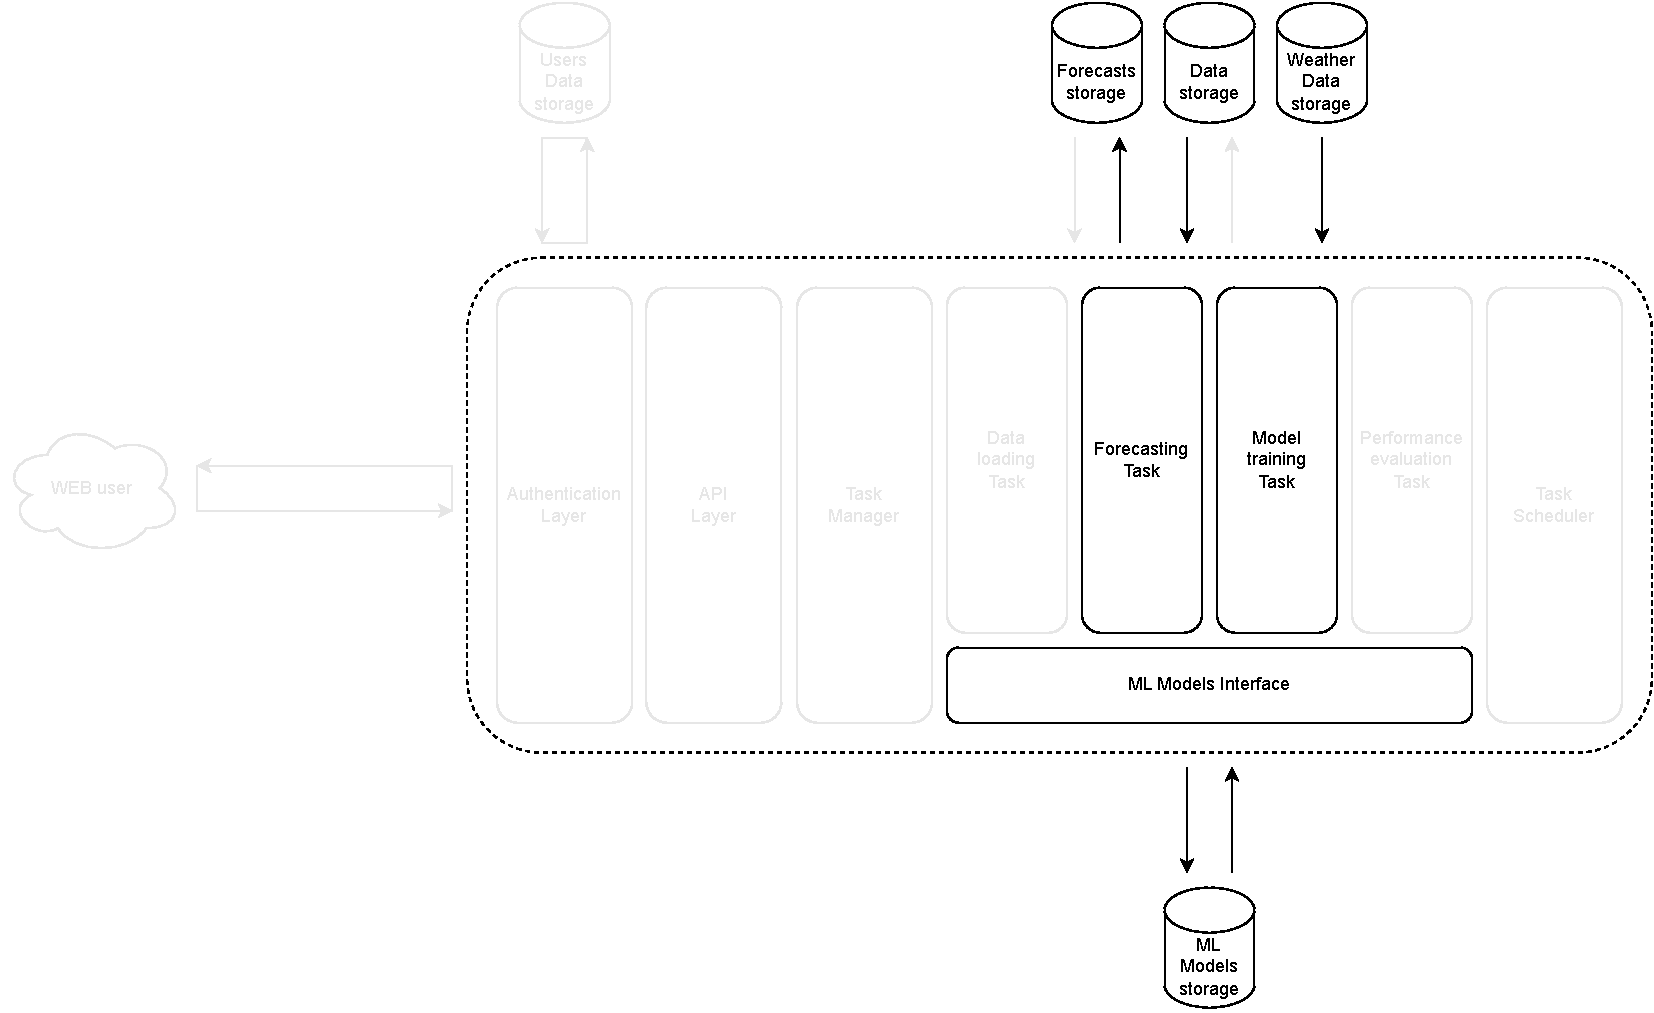
\includegraphics[width=0.9\textwidth]{images/implementation_components}
\caption{The effectively implemented components of the architecture designed for the proposed system.}
\label{fig:implementationcomponents}
\end{figure}

The ML model interface was implemented using the pickle library\footnote{ \url{https://docs.python.org/3/library/pickle.html} } for interfacing with the ML models storage for storing the ML models and retrieving the stored ones making them available for prediction and evaluation.
The use of the MLflow client\footnote{ \url{https://mlflow.org/} } was thought of as a possible interface in the complete system integration for interfacing with the ML models storage.

The model training task trains new models based on available data for the specific use case.
The details about the models and their training process for each specific use case are reported in the dedicated sections.

The forecasting task forecasts future data using the available models for the specific use case.
The details about the models and their forecasting process for each specific use case are reported in the dedicated sections.

The performance evaluation task evaluates the performance of the available models for the specific use case.
The details about the performance evaluation process for each specific use case are reported in chapter~\ref{cha:evaluation}.

\begin{figure}[H]
\centering
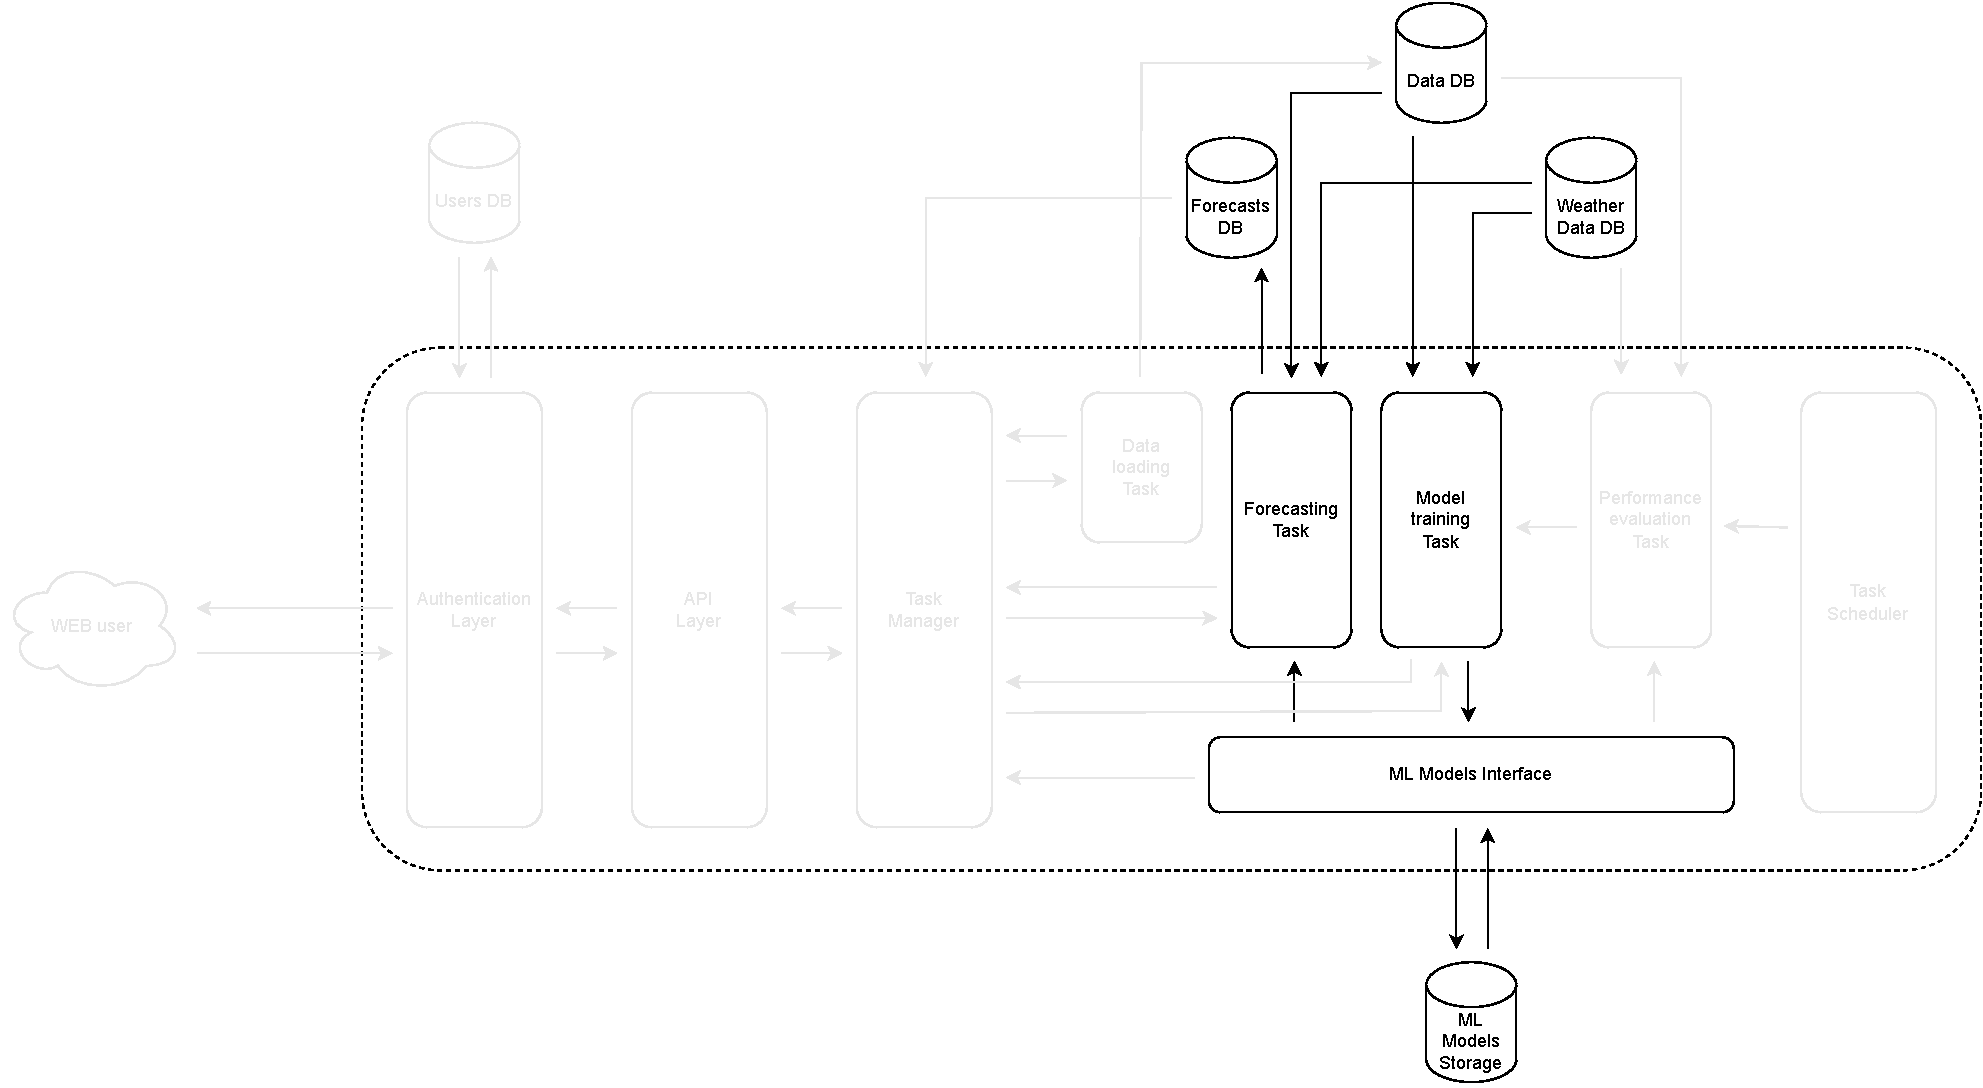
\includegraphics[width=1\textwidth]{images/implementation_interactions}
\caption{The interactions among the effectively implemented components of the architecture designed for the proposed system.}
\label{fig:implementationinteractions}
\end{figure}

The system interacts with the following external components: data storage, weather data storage, ML models storage, and forecasts storage.

The data storage consists of CSV files containing the data for the different use cases, which are loaded using the pandas library\footnote{ \url{https://pandas.pydata.org/} }.
InfluxDB\footnote{ \url{https://www.influxdata.com/} } was thought of as a possible database in the complete system integration for managing the data.

The weather data storage consists of a CSV file and a JSON file containing the weather data, which are loaded using the pandas library.
Weather data in the CSV file is manually obtained from Iowa Environmental Mesonet\footnote{ \url{https://mesonet.agron.iastate.edu/request/download.phtml} } for the weather station in the Murcia airport, and it was used for customers demand forecasting.
Weather data in the JSON file is manually obtained from the Weatherbit\footnote{ \url{https://www.weatherbit.io/} } APIs for a weather station near Murcia airport, these were used for PV plants production forecasting since it provides also solar energy data.
InfluxDB was thought of as a possible database in the complete system integration for managing the weather data with an automatic download of weather data using Weatherbit APIs.

The ML models storage consists of pickle files containing the ML models.
MLflow was thought of as a possible ML model storage in the complete system integration for managing the ML models.

The forecasts storage consists of CSV files containing the forecasts, which are stored using the pandas library.
InfluxDB was thought of as a possible database in the complete system integration for managing the forecasts.


\section{Electricity demand forecasting models}
\label{sec:demandimpl}
\vspace{0.2 cm}

The electricity demand forecasting models rely on dedicated data preprocessing which consists of parsing the aggregated consumption data over the customers from a CSV file using the pandas library.
Then, this basic data is enhanced with the air temperature, the apparent temperature, and the relative humidity parsed from the weather CSV file, in which the reported value is the average of the value in the last hour.
Finally, data is cleaned up by filling in the gaps using the linear interpolation provided by the pandas library, which proved to be effective since there was just some missing data in the weather information.
Two possible granularities are considered: hourly and daily.
The data is with an hourly granularity, so for the daily granularity, data is also aggregated over the day summing the active incomings of the single hours, and averaging the weather data over the day.

The developed models are some baseline approaches that consider repeating past days and weeks, a SARIMA model, a support vector regressor model, a hist gradient boosting regressor model, an extreme gradient boosting regressor model, a prophet model, a LSTM model, a GRU model, a CNN model, some models derived by the combination of the previous techniques, a TFT model, and an AutoML approach.

The baseline approaches are developed using the NumPy library\footnote{ \url{https://numpy.org/} }.
In particular, the tile method is used in different ways depending on the considered baseline.
For the one-day baseline, the last day of the training active incomings is replicated for the days of the test set.
For the one-week baseline, the last week of the training active incomings is replicated for the weeks of the test set.

The SARIMA model is developed using the pmdarima library\footnote{ \url{http://alkaline-ml.com/pmdarima/} }.
The auto\_arima method is used to automatically discover the optimal order for the SARIMA model to better fit the training active incomings using the week as the period for seasonal differencing and in case of the hourly granularity this is done for each hour.
For the prediction, it simply takes in input the length of the test set and computes the predictions.

Support vector regressor and hist gradient boosting regressor models are developed using the scikit-learn library\footnote{ \url{https://scikit-learn.org/} }.
The extreme gradient boosting regressor model is developed using the XGBoost library\footnote{ \url{https://xgboost.readthedocs.io/} }.
Support vector regressor, hist gradient boosting regressor, and extreme gradient boosting regressor models take advantage of the following features for the hourly granularity: the hour, the day, the weekday, the month, and the year information of the time instant for which to compute the prediction, the air temperature, the apparent temperature, and the relative humidity in the considered hour.
In addition, the active incomings of the past 24 hours and the ones of the same hour considered in the previous 14 days are also used.
For the daily granularity instead, the hour information of the date for which to compute the prediction is not considered as a feature, the weather information is obtained as the average over the day, and in place of the active incomings described for the hourly granularity, the daily active incomings of the past 14 days are used.
The training is performed using the fit method on the training data for one-step ahead forecasting.
The specific models' parameters are discussed in the dedicated section of chapter~\ref{cha:evaluation}.
For the prediction, an recursive strategy is used by forecasting one time instant at a time using weather forecasts, and then uaing the predicted demand data as previous information for the next time instants.

The prophet model is developed using the prophet library\footnote{ \url{https://facebook.github.io/prophet/} }.
The fit method tasks as input a pandas data frame with just the information related to the time instants and the training active incomings and fits the optimal prophet model.
For the prediction, it takes as input a pandas data frame with the time instants for which to compute the predictions and computes them, providing also uncertainty intervals.

LSTM, GRU, and CNN models are developed using the Keras library\footnote{ \url{https://keras.io/} }.
These models take advantage of the following features for the hourly granularity: the hour, the day, the weekday, the month, and the year information of the time instant for which to compute the prediction, the air temperature, the apparent temperature, and the relative humidity in the considered hour.
In addition, the active incoming of the previous hour is also used.
Since these models are able to deal with sequences, a look back at the past 3 hours and at the same hour over the past 14 days is considered and passed as input to the models with the same features as the time instant for which to compute the prediction but with the actual consumption data of the past time instants.
For the daily granularity instead, the hour of the date for which to compute the prediction is not considered as a feature, the weather information is obtained as the average over the day, and the considered look back is at the past 14 days.
The training is performed using the fit method on the training data for one-step ahead forecasting.
The specific models' architecture and parameters are discussed in the dedicated section of chapter~\ref{cha:evaluation}.
For the prediction, an recursive strategy is used by forecasting one time instant at a time using weather forecasts, and then uaing the predicted demand data as previous information for the next time instants.

The models derived by the combination of the previous techniques consist of the combination of one-day baseline, one-week baseline, and prophet with possibly one of LSTM, GRU, or CNN.
Further details of the optimal combinations are discussed in the dedicated section of chapter~\ref{cha:evaluation}.

The TFT model is developed using the PyTorch Forecasting library\footnote{ \url{https://pytorch-forecasting.readthedocs.io/} }.
A TimeSeriesDataSet is constructed using the following features for the hourly granularity: the time index, the hour, the day, the weekday, the month, and the year information of the time instant for which to compute the prediction, the air temperature, the apparent temperature, and the relative humidity in the considered hour.
For the daily granularity instead, the hour of the date for which to compute the prediction is not considered as a feature, and the weather information is obtained as the average over the day.
The training is performed using the fit method of the Trainer object provided by the PyTorch Lightning library\footnote{ \url{https://www.pytorchlightning.ai/index.html} } on the training data.
The specific models' parameters are discussed in the dedicated section of chapter~\ref{cha:evaluation}.
For the prediction, it takes as input a TimeSeriesDataSet with the time instants for which to compute the predictions and computes them.

The AutoML approach is based on the TimeSeriesForecastingTask of the Auto-PyTorch library\footnote{ \url{https://automl.github.io/Auto-PyTorch/master/} }.
The AutoML approach takes advantage of the following features for the hourly granularity: the hour, the day, the weekday, the month, and the year information of the time instant for which to compute the prediction, the air temperature, the apparent temperature, and the relative humidity in the considered hour.
For the daily granularity instead, the hour of the date for which to compute the prediction is not considered as a feature, and the weather information is obtained as the average over the day.
The search method is used to search for the best pipeline configuration for the given training data optimizing the machine learning models and building an ensemble out of them.
For the prediction, it takes as input a pandas data frame with the time instants for which to compute the predictions and computes them.


\section{Consumption baseline forecasting models}
\label{sec:baselineimpl}
\vspace{0.2 cm}

The consumption baseline forecasting models rely on dedicated data preprocessing which consists of parsing single customer consumption data from a CSV file using the pandas library.
Then, this basic data is enhanced with the air temperature, the apparent temperature, and the relative humidity parsed from the weather CSV file, in which the reported value is the average of the value in the last hour.
Finally, data is cleaned up by filling in the gaps using the linear interpolation provided by the pandas library, which proved to be effective since there was just some missing data in the weather information.
Three possible granularities are considered: hourly, daily, and by tariff.
The data is with an hourly granularity, so for the daily granularity, data is also aggregated over the day summing the active incomings of the single hours, and averaging the weather data over the day.
The other possible granularity co'nsists in aggregating the data by tariff, in fact, the hourly tariff proposed by MIWenergía is different based on the day and the hour of the day.
For the considered residential users the possible tariffs are 3:
\begin{enumerate}
  \item Working days from 10 AM to 2 PM, and from 6 PM to 10 PM;
  \item Working days from 8 AM to 10 AM, from 2 PM to 6 PM, and from 10 PM to midnight;
  \item Saturday, Sunday, National Holidays, and working days from midnight to 8 AM.
\end{enumerate}
For the tariff granularity, data is aggregated over the day summing the active incomings of the single hours for each tariff, and averaging the weather data over the tariff ranges.

The developed models are some baseline approaches that consider repeating past days and weeks, a SARIMA model, a support vector regressor model, a hist gradient boosting regressor model, an extreme gradient boosting regressor model, a prophet model, a LSTM model, a GRU model, a CNN model, a TFT model, and an AutoML approach.

The baseline approaches are developed using the NumPy library.
In particular, the tile method is used in different ways depending on the considered baseline.
For the one-day baseline, the last day of the training active incomings is replicated for the days of the test set.
For the one-week baseline, the last week of the training active incomings is replicated for the weeks of the test set.
The same was also done considering the average of the previous 4 weeks and of the previous 12 weeks of the training active incomings.

The SARIMA model is developed using the pmdarima library.
The auto\_arima method is used to automatically discover the optimal order for the SARIMA model to better fit the training active incomings using the week as the period for seasonal differencing and in case of the hourly granularity this is done for each hour.
For the prediction, it simply takes in input the length of the test set and computes the predictions.

Support vector regressor and hist gradient boosting regressor models are developed using the scikit-learn library.
The extreme gradient boosting regressor model is developed using the XGBoost library.
Support vector regressor, hist gradient boosting regressor, and extreme gradient boosting regressor models take advantage of the following features for the hourly granularity: the hour, the day, the weekday, the month, and the year information of the time instant for which to compute the prediction, the air temperature, the apparent temperature, and the relative humidity in the considered hour.
In addition, the active incomings of the past 24 hours and the ones of the same hour considered in the previous 14 days are also used.
For the daily and tariff granularities instead, the hour information of the date for which to compute the prediction is not considered as a feature, the weather information is obtained as the average over the day or tariff ranges, and in place of the active incomings described for the hourly granularity, the daily or tariff active incomings of the past 14 days are used.
The training is performed using the fit method on the training data for one-step ahead forecasting.
The specific models' parameters are discussed in the dedicated section of chapter~\ref{cha:evaluation}.
For the prediction, an recursive strategy is used by forecasting one time instant at a time using weather forecasts, and then uaing the predicted demand data as previous information for the next time instants.

The prophet model is developed using the prophet library.
The fit method tasks as input a pandas data frame with just the information related to the time instants and the training active incomings and fits the optimal prophet model.
For the prediction, it takes as input a pandas data frame with the time instants for which to compute the predictions and computes them, providing also uncertainty intervals.

LSTM, GRU, and CNN models are developed using the Keras library.
These models take advantage of the following features for the hourly granularity: the hour, the day, the weekday, the month, and the year information of the time instant for which to compute the prediction, the air temperature, the apparent temperature, and the relative humidity in the considered hour.
In addition, the active incoming of the previous hour is also used.
Since these models are able to deal with sequences, a look back at the past hour and at the same hour over the past 14 days is considered and passed as input to the models with the same features as the time instant for which to compute the prediction but with the actual consumption data of the past time instants.
For the daily and tariff granularities instead, the hour of the date for which to compute the prediction is not considered as a feature, the weather information is obtained as the average over the day or tariff ranges, and the considered look back is at the past 14 days.
The training is performed using the fit method on the training data for one-step ahead forecasting.
The specific models' architecture and parameters are discussed in the dedicated section of chapter~\ref{cha:evaluation}.
For the prediction, an recursive strategy is used by forecasting one time instant at a time using weather forecasts, and then uaing the predicted demand data as previous information for the next time instants.

The TFT model is developed using the PyTorch Forecasting library.
A TimeSeriesDataSet is constructed using the following features for the hourly granularity: the time index, the hour, the day, the weekday, the month, and the year information of the time instant for which to compute the prediction, the air temperature, the apparent temperature, and the relative humidity in the considered hour.
For the daily and tariff granularities instead, the hour of the date for which to compute the prediction is not considered as a feature, and the weather information is obtained as the average over the day or tariff ranges.
The training is performed using the fit method of the Trainer object provided by the PyTorch Lightning library on the training data.
The specific models' parameters are discussed in the dedicated section of chapter~\ref{cha:evaluation}.
For the prediction, it takes as input a TimeSeriesDataSet with the time instants for which to compute the predictions and computes them.

The AutoML approach is based on the TimeSeriesForecastingTask of the Auto-PyTorch library.
The AutoML approach takes advantage of the following features for the hourly granularity: the hour, the day, the weekday, the month, and the year information of the time instant for which to compute the prediction, the air temperature, the apparent temperature, and the relative humidity in the considered hour.
For the daily and tariff granularities granularity instead, the hour of the date for which to compute the prediction is not considered as a feature, and the weather information is obtained as the average over the day or tariff ranges.
The search method is used to search for the best pipeline configuration for the given training data optimizing the machine learning models and building an ensemble out of them.
For the prediction, it takes as input a pandas data frame with the time instants for which to compute the predictions and computes them.


\section{Electricity production forecasting models}
\label{sec:productionimpl}
\vspace{0.2 cm}

The electricity production forecasting models rely on dedicated data preprocessing which consists of parsing single PV plant production data from a CSV file using the pandas library and aggregating the single PV plant data to obtain the aggregated production data over the PV plants.
Then, this basic data is enhanced with the air temperature, the apparent temperature, the relative humidity, the wind speed, the wind direction, the pressure altimeter, the visibility, the sky coverage, the diffuse horizontal irradiance, the direct normal irradiance, the global horizontal irradiance, the solar radiation, the UV index, the solar elevation angle, and the solar azimuth angle parsed from the weather JSON file, in which the reported value is the average of the value in the last hour.
Finally, data is cleaned up by filling in the gaps using the linear interpolation provided by the pandas library, which proved to be effective since there was just some missing data in the weather information.
Only the hourly granularity is considered since PV plants are highly correlated with weather data and the aggregation over the day loses part of this correlation.
The data is with an hourly granularity and the target of the predictions is the mean percentage of production, which is calculated as the division of the total produced energy by the total nominal power of the PV plants.
This allows to have a bounded value from 0 to 100 from which it is possible to obtain the total produced energy simply by multiplying it by the total nominal power of the PV plants.

The developed models are a baseline approach that considers repeating past days, an ARIMA model, a support vector regressor model, a hist gradient boosting regressor model, an extreme gradient boosting regressor model, a prophet model, a LSTM model, a GRU model, a CNN model, some models derived by the combination of the previous techniques, a TFT model, and an AutoML approach.

The baseline approach is developed using the NumPy library.
In particular, the tile method is used.
For the one-day baseline, the last day of the training mean percentages of production is replicated for the days of the test set.

The ARIMA model is developed using the pmdarima library.
The auto\_arima method is used to automatically discover the optimal order for the ARIMA model to better fit the training mean percentages of production and this is done for each hour.
For the prediction, it simply takes in input the length of the test set and computes the predictions.

Support vector regressor and hist gradient boosting regressor models are developed using the scikit-learn library.
The extreme gradient boosting regressor model is developed using the XGBoost library.
Support vector regressor, hist gradient boosting regressor, and extreme gradient boosting regressor models take advantage of the following features: the hour, the day, the weekday, the month, and the year information of the time instant for which to compute the prediction, the air temperature, the apparent temperature, the relative humidity, the diffuse horizontal irradiance, the direct normal irradiance, the global horizontal irradiance, the solar radiation, the UV index, and the solar elevation angle in the considered hour.
In addition, the mean percentages of production of the past 24 hours and the one of the same hour considered in the previous 14 days are also used.
The training is performed using the fit method on the training data for one-step ahead forecasting.
The specific models' parameters are discussed in the dedicated section of chapter~\ref{cha:evaluation}.
For the prediction, an recursive strategy is used by forecasting one time instant at a time using weather forecasts, and then uaing the predicted production data as previous information for the next time instants.

The prophet model is developed using the prophet library.
The fit method tasks as input a pandas data frame with just the information related to the time instants and the training mean percentages of production and fits the optimal prophet model.
For the prediction, it takes as input a pandas data frame with the time instants for which to compute the predictions and computes them, providing also uncertainty intervals.

LSTM, GRU, and CNN models are developed using the Keras library.
These models take advantage of the following features: the hour, the day, the weekday, the month, and the year information of the time instant for which to compute the prediction, the air temperature, the apparent temperature, the relative humidity, the diffuse horizontal irradiance, the direct normal irradiance, the global horizontal irradiance, the solar radiation, the UV index, and the solar elevation angle in the considered hour.
In addition, the mean percentage of production of the previous hour is also used.
Since these models are able to deal with sequences, a look back at the past hour and at the same hour over the past 14 days is considered and passed as input to the models with the same features as the time instant for which to compute the prediction but with the actual production data of the past time instants.
The training is performed using the fit method on the training data for one-step ahead forecasting.
The specific models' architecture and parameters are discussed in the dedicated section of chapter~\ref{cha:evaluation}.
For the prediction, an recursive strategy is used by forecasting one time instant at a time using weather forecasts, and then uaing the predicted production data as previous information for the next time instants.

The models derived by the combination of the previous techniques consist of the combination of one-day baseline and prophet with possibly one of LSTM, GRU, or CNN.
Further details of the optimal combinations are discussed in the dedicated section of chapter~\ref{cha:evaluation}.

The TFT model is developed using the PyTorch Forecasting library.
A TimeSeriesDataSet is constructed using the following features: the time index, the hour, the day, the weekday, the month, and the year information of the time instant for which to compute the prediction, the air temperature, the apparent temperature, the relative humidity, the diffuse horizontal irradiance, the direct normal irradiance, the global horizontal irradiance, the solar radiation, the UV index, and the solar elevation angle in the considered hour.
The training is performed using the fit method of the Trainer object provided by the PyTorch Lightning library\footnote{ \url{https://www.pytorchlightning.ai/index.html} } on the training data.
The specific models' parameters are discussed in the dedicated section of chapter~\ref{cha:evaluation}.
For the prediction, it takes as input a TimeSeriesDataSet with the time instants for which to compute the predictions and computes them.

The AutoML approach is based on the TimeSeriesForecastingTask of the Auto-PyTorch library.
The AutoML approach takes advantage of the following features: the hour, the day, the weekday, the month, and the year information of the time instant for which to compute the prediction, the air temperature, the apparent temperature, the relative humidity, the diffuse horizontal irradiance, the direct normal irradiance, the global horizontal irradiance, the solar radiation, the UV index, and the solar elevation angle in the considered hour.
The search method is used to search for the best pipeline configuration for the given training data optimizing the machine learning models and building an ensemble out of them.
For the prediction, it takes as input a pandas data frame with the time instants for which to compute the predictions and computes them.
